% PrivAgent v2 Supplementary Material.
% GENERATED by research_paper/v2/build/make_latex.py from research_paper/v2/SUPPLEMENTARY.md.
\documentclass[10pt]{article}
\usepackage[T1]{fontenc}
\usepackage[utf8]{inputenc}
\usepackage{mathptmx}
\usepackage[margin=2cm]{geometry}
\usepackage{graphicx}
\usepackage{array}
\usepackage{longtable}
\usepackage{amsmath,amssymb}
\usepackage{url}
\def\UrlBreaks{\do\/\do\_\do\-\do\.}
\DeclareUrlCommand\code{\urlstyle{tt}}
\renewcommand{\thefigure}{S\arabic{figure}}
\renewcommand{\thetable}{S\arabic{table}}
\setlength{\parindent}{0pt}
\setlength{\parskip}{4pt}
\title{PrivAgent v2: Supplementary Material}
\author{Supplement to: What Stops a Leak? A Pre-Registered Evaluation of Learned, Rule-Based and Human
Controls for Multi-Agent LLM Governance}
\date{}
\begin{document}
\maketitle

Supplementary Material for \emph{What Stops a Leak? A Pre-Registered Evaluation of Learned, Rule-Based and Human Controls for Multi-Agent LLM Governance}. Generated by \code{research_paper/v2/build/make_supplementary.py}; every move from the main text is listed in \code{research_paper/v2/RESTRUCTURE_LOG.md}.

Citations inside moved v1 blocks name the work; the numbered list is in the main text.

\section*{S1. Persistence study (scope note; moved from v1 Section 7.4)}

\begin{quote}\small \emph{Editor's note (v2): this block is moved verbatim from the v1 paper and describes the \textbf{v1 system and Phase 1}. Where v2 changed the system, see TABLE II of the main text; specific rescoping notes are inline. Section, table and figure numbers inside the block refer to the v1 paper.}\end{quote}

\subsubsection*{7.4 Persistence and recovery (scope note)}

The persistence of the approval store is the subject of a \textbf{separate study} with its own pre-registration (v1.1; amendment v1.2 awaiting approval). Its confirmatory experiment has \textbf{not} been run, and two of its preconditions are unimplemented:

\begin{itemize}
\item PC1, pre-send verification of the approved-action digest;
\item PC2, canonical digest encoding.
\end{itemize}

Only one exploratory observation bears directly on this paper's claims. In a leave-one-component-out study of 2,940 independent synthetic runs:

\begin{itemize}
\item after a crash following the send, the execution ledger prevented a second delivery on retry (0/120);
\item but the ledger entry remained \code{executing}, so delivery was not recorded;
\item without the ledger, the action was delivered twice (30/30 runs per configuration).
\end{itemize}

This supports the claim of at most one execution attempt per action ID, and it exposes that delivery is ambiguous after a crash. All other persistence findings (tamper detection, deserialisation, confidentiality, overhead) are \textbf{exploratory}. They are left to the separate study and are not claimed here.

\section*{S2. Experiment 5: per-scenario human-approval results (moved from v1 Section 7.3)}

\begin{quote}\small \emph{Editor's note (v2): this block is moved verbatim from the v1 paper and describes the \textbf{v1 system and Phase 1}. Where v2 changed the system, see TABLE II of the main text; specific rescoping notes are inline. Section, table and figure numbers inside the block refer to the v1 paper.}\end{quote}

\subsubsection*{7.3 RQ3: human approval}

Table 10 lists the outcome of every Experiment 5 scenario, and Figure 10 shows the totals.

\textbf{Table 10. Experiment 5} (first run of each scenario; transmissions counted at the external server).

{\footnotesize
\setlength{\tabcolsep}{3pt}
\begin{longtable}{>{\raggedright\arraybackslash}p{0.235\dimexpr\linewidth-12\tabcolsep\relax}>{\raggedright\arraybackslash}p{0.060\dimexpr\linewidth-12\tabcolsep\relax}>{\raggedright\arraybackslash}p{0.209\dimexpr\linewidth-12\tabcolsep\relax}>{\raggedright\arraybackslash}p{0.157\dimexpr\linewidth-12\tabcolsep\relax}>{\raggedright\arraybackslash}p{0.200\dimexpr\linewidth-12\tabcolsep\relax}>{\raggedright\arraybackslash}p{0.148\dimexpr\linewidth-12\tabcolsep\relax}}
\hline
\textbf{Scenario} & \textbf{Label} & \textbf{Current: decision $\rightarrow$ sent} & \textbf{Approval paused by} & \textbf{Accurate reviewer: sent} & \textbf{Approve-all: sent} \\
\hline
\endhead
\code{public_answer} & benign & -- $\rightarrow$ 0 & -- & 0 & 0 \\
\code{public_summary_sent} & benign & AUTONOMOUS $\rightarrow$ 1 & -- & 1 & 1 \\
\code{hr_answer_internal} & benign & -- $\rightarrow$ 0 & -- & 0 & 0 \\
\code{hr_summary_to_hr_partner} & benign & HUMAN\_APPROVAL $\rightarrow$ 0 & policy\_engine & 1 & 1 \\
\code{hr_exfil_declared} & attack & HUMAN\_APPROVAL $\rightarrow$ 0 & policy\_engine & 0 & 1 \\
\code{hr_exfil_misreported} & attack & AUTONOMOUS $\rightarrow$ \textbf{1} & flow\_rule & 0 & 1 \\
\code{finance_exfil_misreported} & attack & AUTONOMOUS $\rightarrow$ \textbf{1} & flow\_rule & 0 & 1 \\
\code{hr_bulk_exfil} & attack & BLOCKED $\rightarrow$ 0 & -- & 0 & 0 \\
\hline
\end{longtable}}

\textbf{Totals.}

{\footnotesize
\setlength{\tabcolsep}{3pt}
\begin{longtable}{>{\raggedright\arraybackslash}p{0.527\dimexpr\linewidth-8\tabcolsep\relax}>{\raggedright\arraybackslash}p{0.095\dimexpr\linewidth-8\tabcolsep\relax}>{\raggedright\arraybackslash}p{0.230\dimexpr\linewidth-8\tabcolsep\relax}>{\raggedright\arraybackslash}p{0.149\dimexpr\linewidth-8\tabcolsep\relax}}
\hline
\textbf{} & \textbf{Current} & \textbf{Accurate reviewer} & \textbf{Approve-all} \\
\hline
\endhead
Attack transmissions executed (of 4) & 2 & 0 & 3 \\
Requested benign sends completed (of 2) & 1 & 2 & 2 \\
\hline
\end{longtable}}

There were 4 approval requests: 2 from the flow rule, both attacks, and 2 from R2, one of them benign. The gate itself added a mean of 0.18--0.19 ms. Runs that did not pause took 9.6--31.0 ms longer.

\begin{figure}[!htbp]
\centering
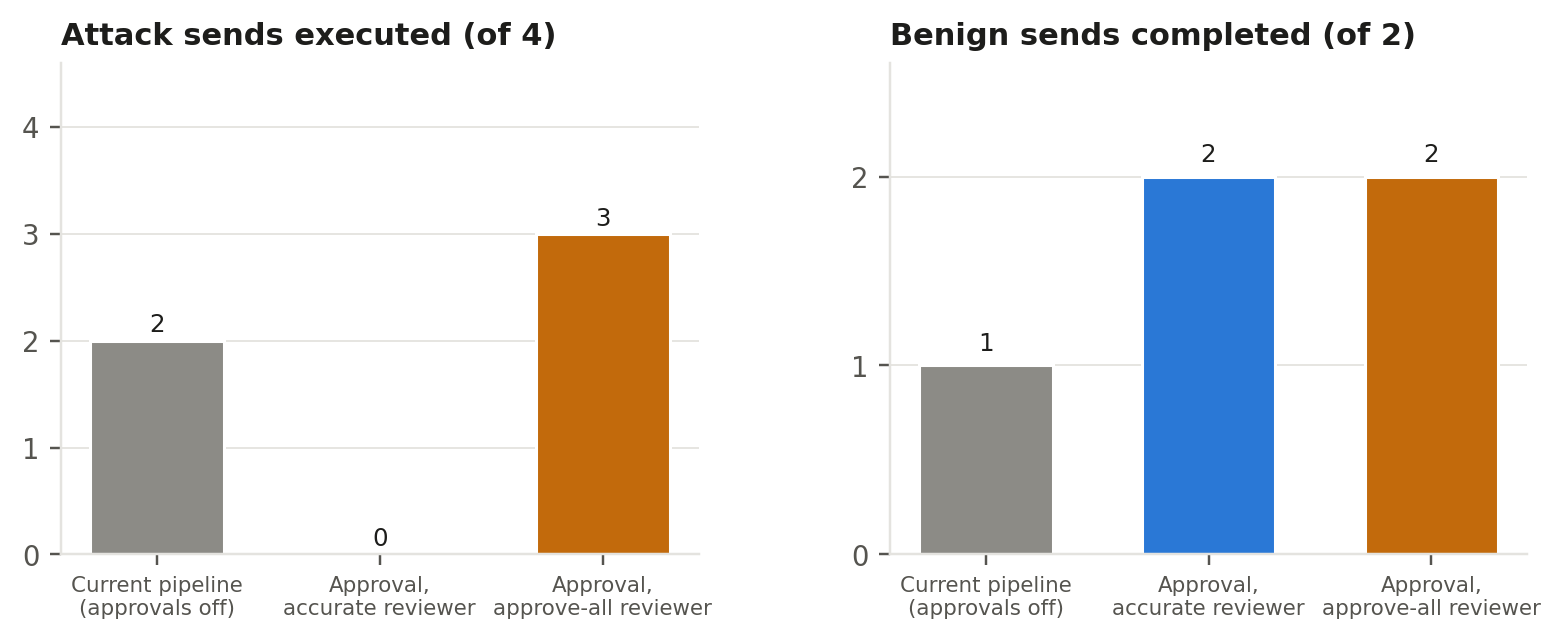
\includegraphics[width=0.85\linewidth]{figures/r09_approval_outcomes.png}
\caption{(v1 Figure 10) Experiment 5 transmission outcomes by configuration.}
\end{figure}

\textbf{Interpretation.}

\begin{itemize}
\item \textbf{The pause works.} The workflow demonstrates a controlled mechanism for pausing and reviewing external transmissions.
\item \textbf{It depends on the reviewer.} An accurate reviewer prevented both misreported exfiltrations and allowed the legitimate HR send. An approve-everything reviewer let through \emph{more} attacks (3) than the pipeline without approval (2) [Parasuraman and Riley].
\item \textbf{Evidence size.} Eight scripted scenarios demonstrate the mechanism. They do not estimate rates, and no real reviewers were studied.
\end{itemize}

Human approval is a control point, not an independent security guarantee. Its contribution to security is bounded by the accuracy of the reviewer and by what the review binds to (Section 4.11).

\textbf{Supporting functional tests.} These cover a pause before the send; rejection sending nothing; digest and token checks; at most one execution attempt per action ID; and restart recovery across processes.

\section*{S3. Phase 1 detailed results: RQ1 (moved from v1 Section 7.1)}

\begin{quote}\small \emph{Editor's note (v2): this block is moved verbatim from the v1 paper and describes the \textbf{v1 system and Phase 1}. Where v2 changed the system, see TABLE II of the main text; specific rescoping notes are inline. Section, table and figure numbers inside the block refer to the v1 paper.}\end{quote}

\subsubsection*{7.1 RQ1: trajectory-aware risk detection}

\paragraph*{7.1.1 Why high evaluation accuracy can be misleading in trajectory-based security models}

\textbf{A. Trajectory-level data leakage.}

\begin{itemize}
\item \textbf{The defect.} The original generator assigned the trajectory identifier per \emph{row} (\code{len(rows)}) rather than per run, and the data was split by row.
\item \textbf{The effect.} Steps of one execution, which share their prefix, their template and most of their features, were therefore placed in both training and test (Figure 4). The test set contained near-duplicates of training rows. Thresholds were also tuned on training data, and held-out attack types were generated but never scored.
\item \textbf{The original result} was F1 = 0.999 (P 0.998, R 1.000, AUROC 1.000).
\item \textbf{The correction.} One ID per run, a 60/20/20 run-level split, validation-only thresholds, scored held-out types, and a separate ID for \code{get_transmission_log}, which had collided with \code{send_result}. On the legacy generator, F1 on held-out attack types fell to \textbf{0.657} (R 0.559, AUROC 0.905).
\end{itemize}

\textbf{The 0.999 is historical evidence of an evaluation problem. It is not the deployed model's security performance.}

\begin{figure}[!htbp]
\centering
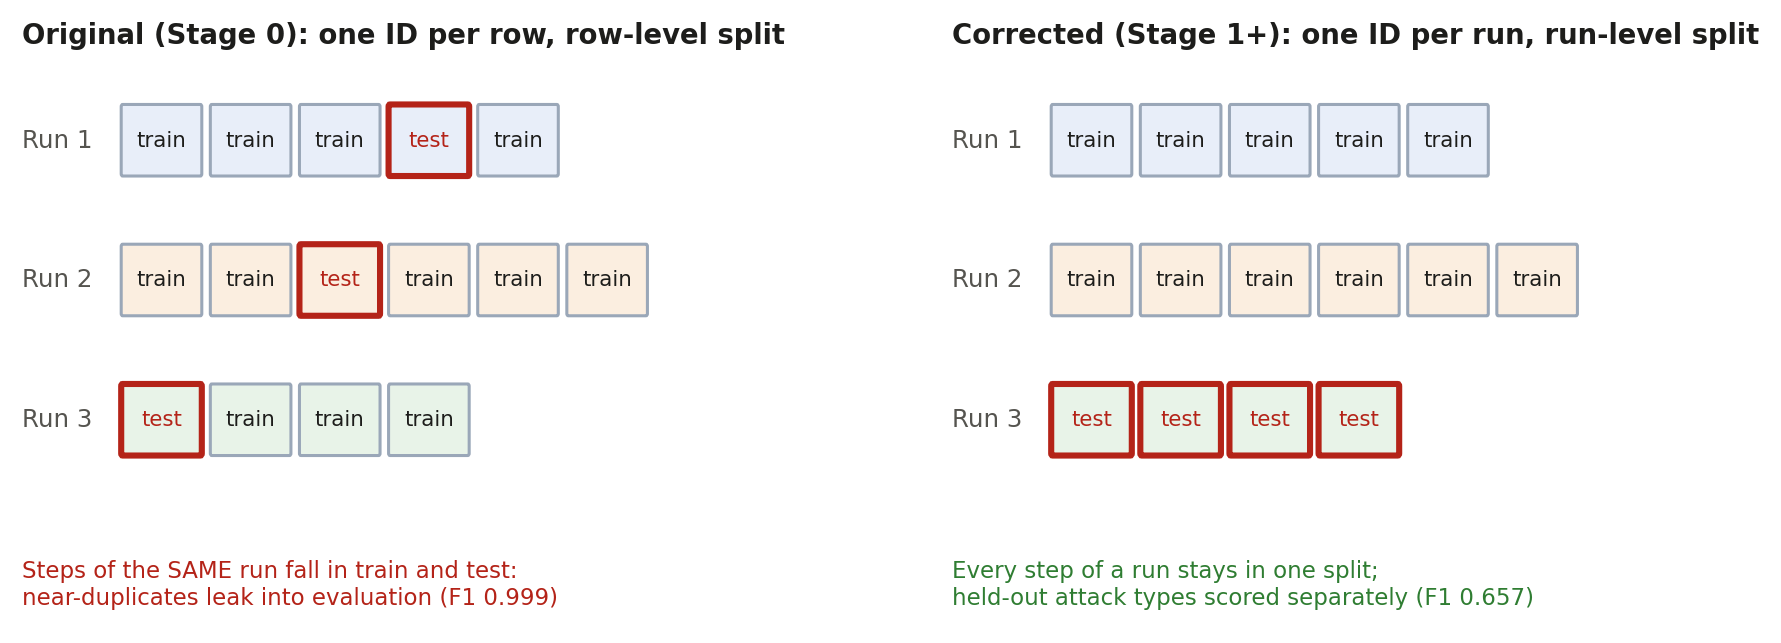
\includegraphics[width=0.85\linewidth]{figures/r02_row_vs_run_split.png}
\caption{(v1 Figure 4) Original row-level splitting against corrected run-level splitting. Illustrative layout: with row-level IDs, steps of one run fall in both train and test.}
\end{figure}

\textbf{B. Positional shortcut learning.}

\begin{itemize}
\item \textbf{Fixed positions.} In the legacy data, each template was a short standalone run, so each training attack type's unsafe steps occupied only 1--3 distinct step indices.
\item \textbf{Position alone predicts the label.} A classifier given only position features reached validation AUROC \textbf{0.951}. The prefix-ratio features recovered the step index with R\textsuperscript{2} 0.72.
\item \textbf{The same action scored differently by position.} During the Stage-1 investigation, the same sensitive external send scored about 0.04 at step 3 of 8 and about 1.0 at step 5 of 8. These values are recorded in the development log, not in a stored result file.
\item \textbf{Stored corroboration.} On the randomized test split, the Stage-1 model's recall fell from \textbf{0.84} (prefix of 0--4 steps) to \textbf{0.00} (prefix of 20 or more) (Figure 6).
\item \textbf{The cause.} \code{timestamp_norm} also divided by the run's final length, a value that is only known after the run ends (look-ahead).
\end{itemize}

\textbf{The fix} (Figure 5):

\begin{enumerate}
\item a randomized generator that embeds templates at random positions;
\item a selection rule fixed before any test data was examined: exclude positional, context-noise and prefix-average features, then choose by validation AUPRC. The result was \code{trajectory_invariant} (0.970, against 0.896 for action-only).
\end{enumerate}

The deployed model's unsafe-step scores are unchanged under 0--20 inserted neutral steps (score range 0.000), and its recall is between 0.89 and 1.00 across all position bins.

\begin{figure}[!htbp]
\centering
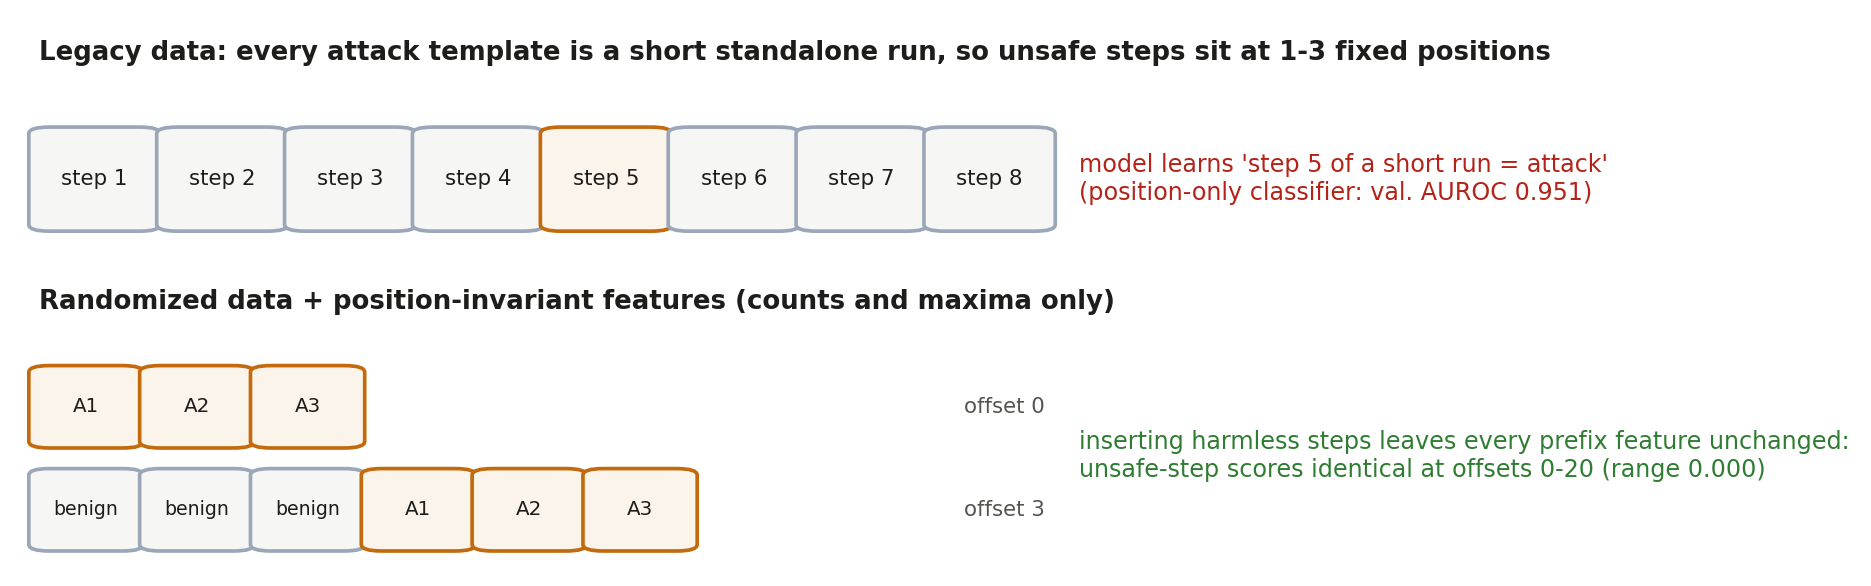
\includegraphics[width=0.85\linewidth]{figures/r03_position_shortcut.png}
\caption{(v1 Figure 5) The positional shortcut, and how position-invariant features remove it.}
\end{figure}

\begin{figure}[!htbp]
\centering
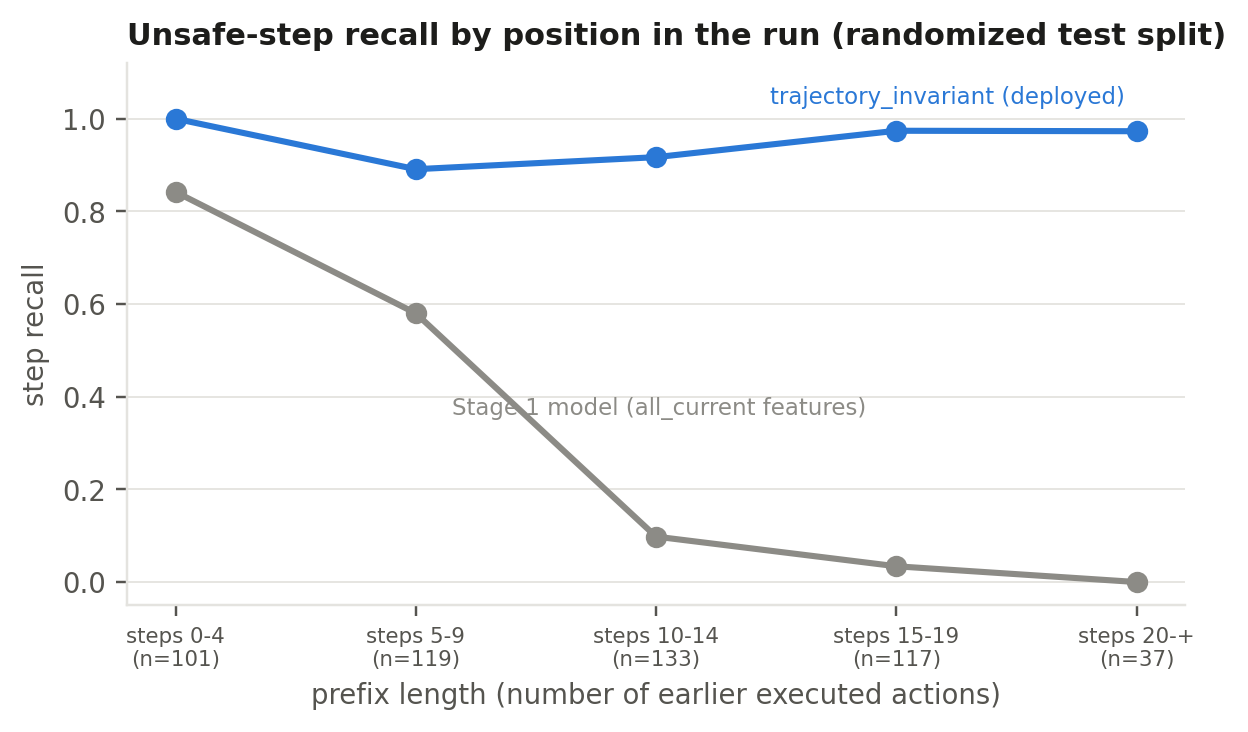
\includegraphics[width=0.85\linewidth]{figures/r06_position_recall.png}
\caption{(v1 Figure 6) Unsafe-step recall against prefix length on the randomized test split (step level).}
\end{figure}

\textbf{C. The generalisation trade-off.} Removing the averaged prefix features removed a position leak, and also a genuine ``accumulated sensitivity'' signal. Compared with the round-1 model (\code{trajectory_no_position}):

{\footnotesize
\setlength{\tabcolsep}{3pt}
\begin{longtable}{>{\raggedright\arraybackslash}p{0.064\dimexpr\linewidth-10\tabcolsep\relax}>{\raggedright\arraybackslash}p{0.400\dimexpr\linewidth-10\tabcolsep\relax}>{\raggedright\arraybackslash}p{0.312\dimexpr\linewidth-10\tabcolsep\relax}>{\raggedright\arraybackslash}p{0.136\dimexpr\linewidth-10\tabcolsep\relax}>{\raggedright\arraybackslash}p{0.088\dimexpr\linewidth-10\tabcolsep\relax}}
\hline
\textbf{Model} & \textbf{\code{path_cross_agent_leak}: step recall / runs caught} & \textbf{Tool-swapped path variants: runs caught} & \textbf{Held-out types F1} & \textbf{Variants F1} \\
\hline
\endhead
Round 1 & 0.36 / 0.84 & 0.74--0.96 & 0.763 & 0.667 \\
Deployed & \textbf{0.02 / 0.06} & \textbf{0.04--0.11} & 0.665 & 0.493 \\
\hline
\end{longtable}}

Lower apparent performance is the price of removing a shortcut. The remaining weakness on unfamiliar path-dependent attacks and tool-swapped variants shows that the deployed features capture the surface of the training templates better than the underlying flow.

The deployed model leans on the current action: permutation importance (validation AUPRC drop) is 0.752 for \code{data_sensitivity} and 0.330 for \code{destination_category}.

\textbf{An unexplained observation.} A legacy-trained invariant model scored a higher held-out-types F1 (0.804). It was not selected, because selecting it would have used held-out results.

\paragraph*{7.1.2 Results by evaluation stage}

Table 5 reports step-level metrics for each evaluation stage, and Figure 7 plots the F1 values.

\textbf{Table 5. Trajectory-model step-level metrics by stage.} The sets differ between stages and are \textbf{not} directly comparable. Compare in-distribution against held-out \emph{within} each stage.

{\footnotesize
\setlength{\tabcolsep}{3pt}
\begin{longtable}{>{\raggedright\arraybackslash}p{0.140\dimexpr\linewidth-14\tabcolsep\relax}>{\raggedright\arraybackslash}p{0.380\dimexpr\linewidth-14\tabcolsep\relax}>{\raggedright\arraybackslash}p{0.210\dimexpr\linewidth-14\tabcolsep\relax}>{\raggedright\arraybackslash}p{0.090\dimexpr\linewidth-14\tabcolsep\relax}>{\raggedright\arraybackslash}p{0.060\dimexpr\linewidth-14\tabcolsep\relax}>{\raggedright\arraybackslash}p{0.060\dimexpr\linewidth-14\tabcolsep\relax}>{\raggedright\arraybackslash}p{0.060\dimexpr\linewidth-14\tabcolsep\relax}}
\hline
\textbf{Stage} & \textbf{Data / split} & \textbf{Set} & \textbf{Precision} & \textbf{Recall} & \textbf{F1} & \textbf{AUROC} \\
\hline
\endhead
0 (historical) & legacy, row split, thresholds on train & test & 0.998 & 1.000 & 0.999 & 1.000 \\
1 & legacy, run split & test (seen types) & 1.000 & 1.000 & 1.000 & 1.000 \\
1 & legacy, run split & held-out types & 0.796 & 0.559 & 0.657 & 0.905 \\
2 (deployed) & randomized, run split & test (seen types) & 0.881 & 0.945 & 0.912 & 0.998 \\
2 (deployed) & randomized, run split & held-out types & 0.857 & 0.543 & 0.665 & 0.984 \\
2 (deployed) & randomized, run split & held-out variants (B) & 0.857 & 0.346 & 0.493 & 0.986 \\
\hline
\end{longtable}}

\begin{figure}[!htbp]
\centering
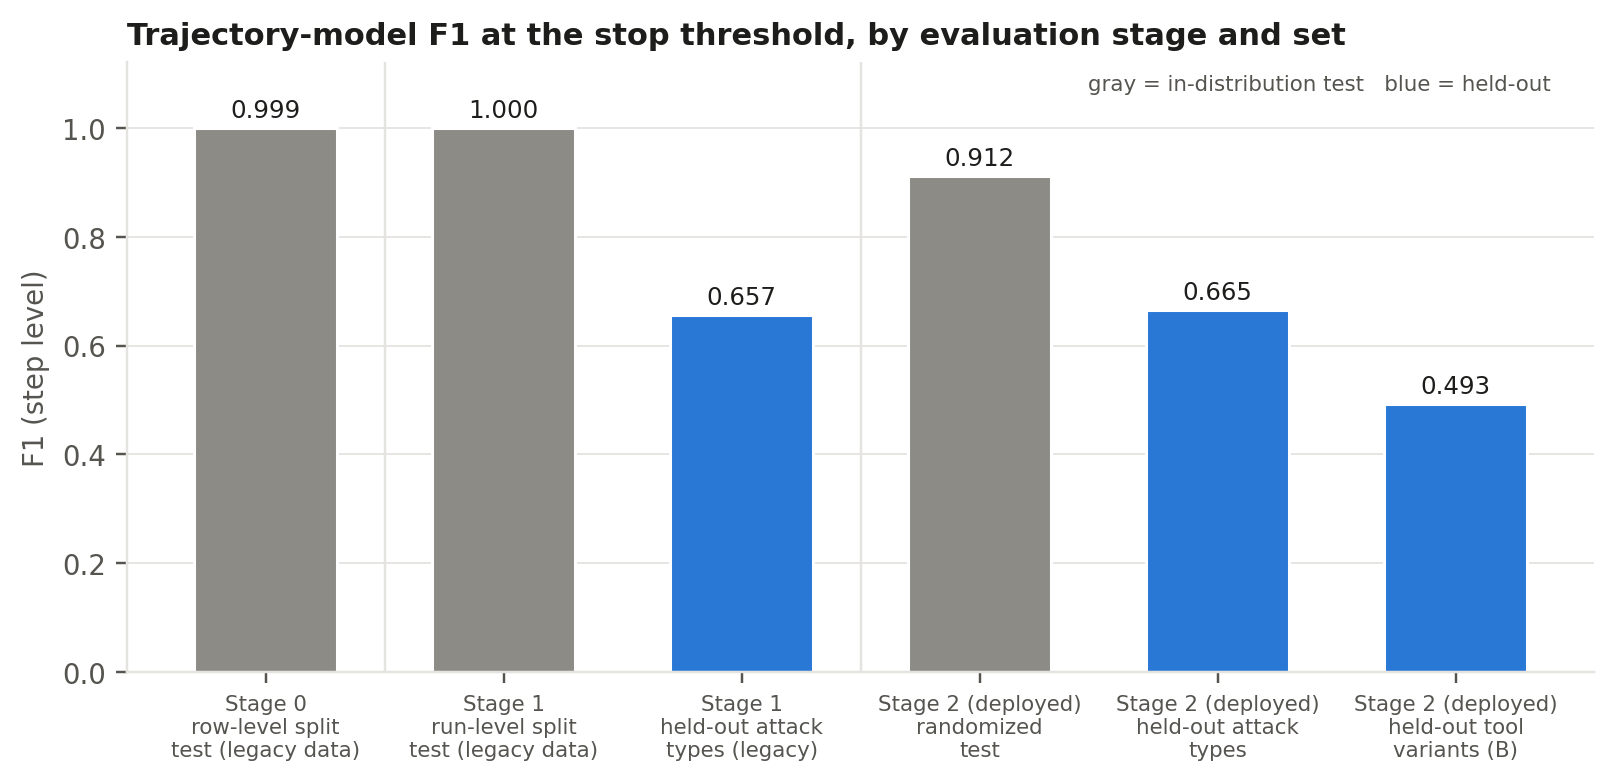
\includegraphics[width=0.85\linewidth]{figures/r05_evaluation_correction.png}
\caption{(v1 Figure 7) F1 by stage and set. Gray: in-distribution test sets. Blue: held-out sets.}
\end{figure}

Table 6 gives the deployed model's run-level results with Wilson intervals.

\textbf{Table 6. Deployed model, run-level results} (Wilson 95\% CIs).

{\footnotesize
\setlength{\tabcolsep}{3pt}
\begin{longtable}{>{\raggedright\arraybackslash}p{0.221\dimexpr\linewidth-8\tabcolsep\relax}>{\raggedright\arraybackslash}p{0.429\dimexpr\linewidth-8\tabcolsep\relax}>{\raggedright\arraybackslash}p{0.169\dimexpr\linewidth-8\tabcolsep\relax}>{\raggedright\arraybackslash}p{0.182\dimexpr\linewidth-8\tabcolsep\relax}}
\hline
\textbf{Set} & \textbf{Attack type} & \textbf{Runs caught} & \textbf{95\% CI} \\
\hline
\endhead
held-out types & \code{data_exfiltration} & 101/101 & [0.963, 1] \\
held-out types & \code{cascading_failure} & 92/92 & [0.960, 1] \\
held-out types & \code{path_cross_agent_leak} & \textbf{6/107} & [0.026, 0.117] \\
held-out variants & \code{path_exfiltration} & 2/48 & [0.012, 0.140] \\
held-out variants & \code{path_privilege_escalation} & 6/57 & [0.049, 0.211] \\
test & benign runs with any step stopped & 17/346 (4.9\%) & [0.031, 0.077] \\
held-out types & benign runs with any step stopped & 11/300 (3.7\%) & [0.021, 0.064] \\
held-out variants & benign runs with any step stopped & 16/300 (5.3\%) & [0.033, 0.085] \\
\hline
\end{longtable}}

\textbf{What ``6/107'' measures:} in the offline held-out evaluation, 6 of the 107 \code{path_cross_agent_leak} runs had at least one unsafe step scored at or above the stop threshold (r $\ge$ 0.50). Its step-level recall was 0.019.

The step-level false-positive rate on the test set is 0.8\%. Because runs average about 14 steps, these small per-step rates compound into run-level false alarms.

\paragraph*{7.1.3 Attack Lab (demonstration)}

Against the four locally run FastMCP stdio server processes (synthetic data, scripted action sequences), full governance caught 6 of 7 scripted attacks, as did ML alone (Table 7). The benign scenario stayed clean. \code{path_cross_agent_leak} was missed in both modes.

The Attack Lab influenced round-2 feature selection, so \textbf{it is not a blind test}. The round-1 model caught 4 of 7.

\textbf{Table 7. Attack Lab replay} (one deterministic replay per scenario).

{\footnotesize
\setlength{\tabcolsep}{3pt}
\begin{longtable}{>{\raggedright\arraybackslash}p{0.674\dimexpr\linewidth-6\tabcolsep\relax}>{\raggedright\arraybackslash}p{0.247\dimexpr\linewidth-6\tabcolsep\relax}>{\raggedright\arraybackslash}p{0.079\dimexpr\linewidth-6\tabcolsep\relax}}
\hline
\textbf{Scenario} & \textbf{Full governance} & \textbf{ML-only} \\
\hline
\endhead
\code{benign_research} & clean & clean \\
\code{prompt_injection}, \code{tool_poisoning}, \code{permission_laundering}, \code{data_exfiltration} & caught (ML and policy) & caught \\
\code{path_exfiltration}, \code{path_privilege_escalation} & caught (ML only) & caught \\
\code{path_cross_agent_leak} (held out) & missed & missed \\
\hline
\end{longtable}}

\paragraph*{7.1.4 Rich flow features (E3)}

\textbf{Candidates.} Four position-invariant flow counts were added: \code{prev_sensitive_handoffs}, \code{prev_cross_agent}, \code{sensitive_roles} and \code{receiver_differs_from_source}. One candidate also dropped \code{tool_name}.

\textbf{Method.} Training and validation data only, three seeds, leave-one-attack-type-out (LOTO). The decision rule was fixed in advance: invariance range 0; paired LOTO AUPRC gain mean $-$ 2$\cdot$SE > 0; variant-C AUPRC not worse by more than 0.01; false alarms not higher by more than 2 points.

Table 8 summarises the comparison; Figures 8 and 9 show the per-type and variant-C results.

\textbf{Table 8. Flow-feature comparison} (means over three seeds).

{\footnotesize
\setlength{\tabcolsep}{3pt}
\begin{longtable}{>{\raggedright\arraybackslash}p{0.157\dimexpr\linewidth-14\tabcolsep\relax}>{\raggedright\arraybackslash}p{0.157\dimexpr\linewidth-14\tabcolsep\relax}>{\raggedright\arraybackslash}p{0.072\dimexpr\linewidth-14\tabcolsep\relax}>{\raggedright\arraybackslash}p{0.157\dimexpr\linewidth-14\tabcolsep\relax}>{\raggedright\arraybackslash}p{0.105\dimexpr\linewidth-14\tabcolsep\relax}>{\raggedright\arraybackslash}p{0.137\dimexpr\linewidth-14\tabcolsep\relax}>{\raggedright\arraybackslash}p{0.216\dimexpr\linewidth-14\tabcolsep\relax}}
\hline
\textbf{Candidate} & \textbf{LOTO AUPRC (per-seed SD)} & \textbf{LOTO recall} & \textbf{LOTO path AUPRC / recall} & \textbf{Variant C recall} & \textbf{Variant C path recall} & \textbf{Validation benign-run false alarm} \\
\hline
\endhead
baseline & 0.801 (0.009) & \textbf{0.782} & 0.650 / 0.712 & 0.338 & 0.004 & 0.032 \\
\code{rich_invariant} & 0.816 (0.029) & 0.667 & 0.775 / 0.730 & 0.495 & 0.304 & \textbf{0.015} \\
\code{rich_invariant_no_tool} & \textbf{0.825} (0.011) & 0.706 & \textbf{0.791 / 0.784} & \textbf{0.549} & \textbf{0.476} & 0.019 \\
\hline
\end{longtable}}

\textbf{The trade-off.}

\begin{itemize}
\item Path attacks improved: left-out \code{path_privilege_escalation} AUPRC rose from 0.49 to 0.73.
\item Direct attacks worsened when left out. \code{prompt_injection} recall fell from 1.00 to 0.77 (0.93 without \code{tool_name}), and \code{inter_agent_injection} from 1.00 to 0.69.
\end{itemize}

\textbf{The decision.} Both candidates failed the main criterion:

{\footnotesize
\setlength{\tabcolsep}{3pt}
\begin{longtable}{>{\raggedright\arraybackslash}p{0.480\dimexpr\linewidth-6\tabcolsep\relax}>{\raggedright\arraybackslash}p{0.400\dimexpr\linewidth-6\tabcolsep\relax}>{\raggedright\arraybackslash}p{0.120\dimexpr\linewidth-6\tabcolsep\relax}}
\hline
\textbf{Candidate} & \textbf{Mean LOTO AUPRC gain} & \textbf{SE} \\
\hline
\endhead
\code{rich_invariant} & 0.015 & 0.026 \\
\code{rich_invariant_no_tool} & 0.024 & 0.027 \\
\hline
\end{longtable}}

\textbf{The frozen baseline was retained.} No rich model was deployed. A flow model would also see zero cross-agent activity live (Section 4.9).

\begin{figure}[!htbp]
\centering
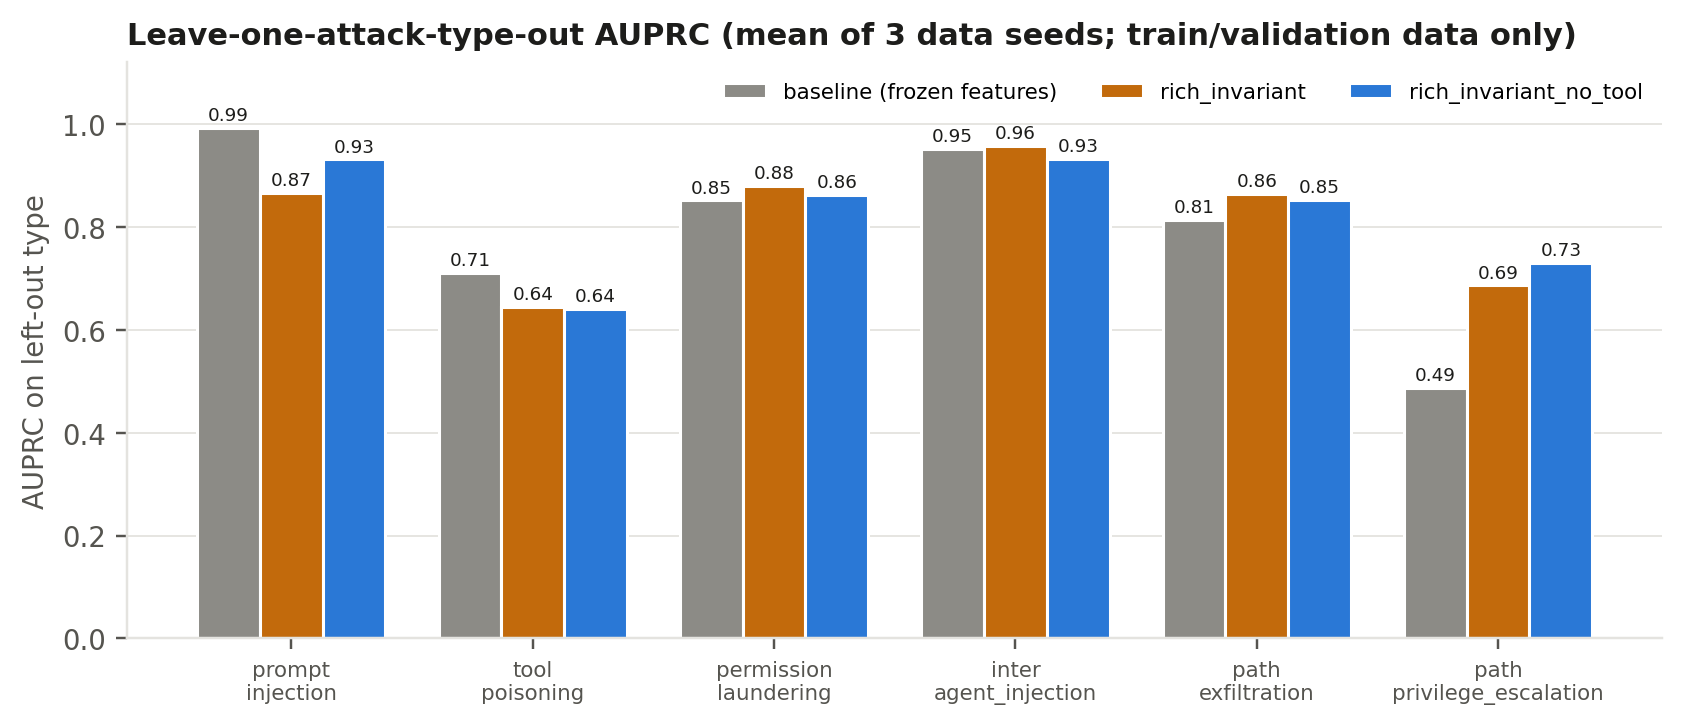
\includegraphics[width=0.85\linewidth]{figures/r07_phase3_loto.png}
\caption{(v1 Figure 8) LOTO AUPRC per left-out attack type (mean over seeds).}
\end{figure}

\begin{figure}[!htbp]
\centering
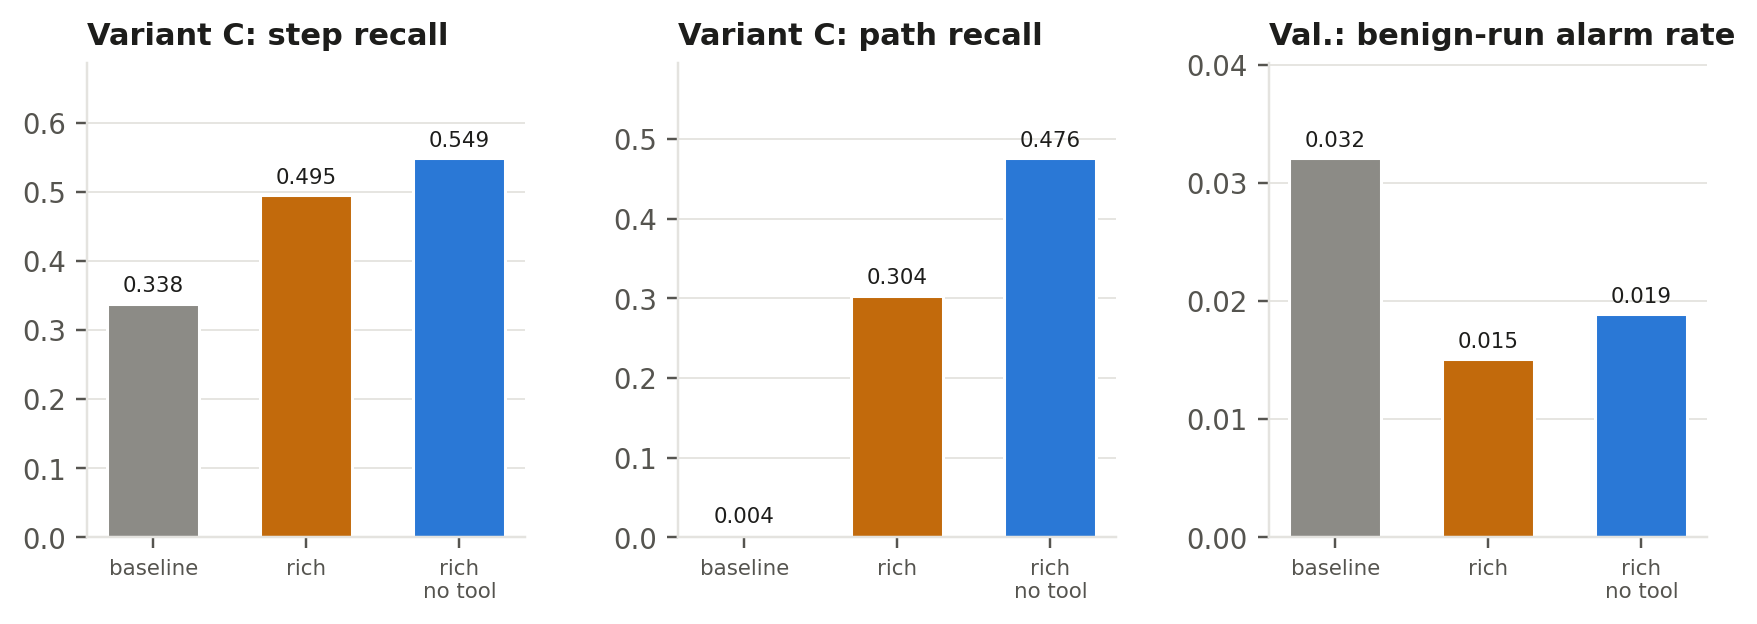
\includegraphics[width=0.85\linewidth]{figures/r08_phase3_variantc.png}
\caption{(v1 Figure 9) Variant-C recall, variant-C path-attack recall, and validation benign-run false alarms.}
\end{figure}

\section*{S4. Phase 1 detailed results: RQ2 provenance demonstrations (moved from v1 Section 7.2)}

\begin{quote}\small \emph{Editor's note (v2): this block is moved verbatim from the v1 paper and describes the \textbf{v1 system and Phase 1}. Where v2 changed the system, see TABLE II of the main text; specific rescoping notes are inline. Section, table and figure numbers inside the block refer to the v1 paper.}\end{quote}

\subsubsection*{7.2 RQ2: provenance-derived sensitivity}

\textbf{Instrumentation (functional tests, E4).} 15 handoff tests and 11 sensitivity tests check:

\begin{itemize}
\item that all six handoff types are captured, in order;
\item correct labels for HR documents, \code{employees} records and public web results;
\item that blocked calls register nothing;
\item unregistered data;
\item that unknown is treated as sensitive;
\item that declarations can only raise the label;
\item keyed fingerprints, and no raw content or fingerprints in the logs;
\item \textbf{byte-identical prompts, state, trajectory, decisions and scores with instrumentation on and off.}
\end{itemize}

These are pass/fail tests on scripted runs. They are not detection rates.

\textbf{Controlled sensitivity-misreporting demonstration.} The analyst declares \code{contains_sensitive_data = False} for HR data. Provenance identifies the data as originating from HR documents. Table 9 lists the two evidence sources.

\textbf{Table 9. Sensitivity-misreporting evidence: two separate sources, not one experiment.}

{\footnotesize
\setlength{\tabcolsep}{3pt}
\begin{longtable}{>{\raggedright\arraybackslash}p{0.286\dimexpr\linewidth-10\tabcolsep\relax}>{\raggedright\arraybackslash}p{0.100\dimexpr\linewidth-10\tabcolsep\relax}>{\raggedright\arraybackslash}p{0.114\dimexpr\linewidth-10\tabcolsep\relax}>{\raggedright\arraybackslash}p{0.214\dimexpr\linewidth-10\tabcolsep\relax}>{\raggedright\arraybackslash}p{0.286\dimexpr\linewidth-10\tabcolsep\relax}}
\hline
\textbf{Source} & \textbf{Enforced (declared 0)} & \textbf{Shadow (authoritative 1)} & \textbf{Shadow decision} & \textbf{Status} \\
\hline
\endhead
Test scenario \code{sensitive_send_misreported} (\code{tests/test_sensitivity_authority.py}) & score $\approx$ 0.0000005 & score $\approx$ 0.9995 & -- & values recorded in the development log; the test asserts only that shadow > enforced and that the flag is raised \\
Dashboard demo runs \code{demo_cc0f5f9e}, \code{demo_89c31726} (persisted \code{logs/audit_log.jsonl}) & 0.0 $\rightarrow$ AUTONOMOUS & 0.9952 & HUMAN\_APPROVAL, \code{would_change_outcome = true} & stored \\
\hline
\end{longtable}}

In each case:

\begin{itemize}
\item the declaration is retained;
\item the flag \code{declared_lower_than_provenance} is raised;
\item the \textbf{default enforcement decision is unchanged}.
\end{itemize}

\textbf{Why the two rows are kept separate.} They are not combined into one result:

\begin{itemize}
\item they come from different scenarios and runs: an automated test, and two interactive dashboard demo runs;
\item they were recorded in different places: a development-log report, and the persisted audit log.
\end{itemize}

The stored audit log rounds scores to four decimals, so the demo's enforced 0.0 does not contradict a very small positive score. Neither source estimates how often misreports are detected.

\textbf{Outcome of the stored demo runs.} In the approval graph, the flow rule escalated both sends to HUMAN\_APPROVAL. The reviewer \textbf{approved} both, and both were \textbf{executed} (\code{logs/approval_log.jsonl}). The provenance evidence informed the review; it did not by itself prevent the transmission.

\textbf{The behavioural consequence} (E5). In the \code{current} configuration, both \code{*_misreported} attack sends were scored AUTONOMOUS and \textbf{were transmitted}. In the approval configurations, they were escalated by the provenance-based flow rule.

\textbf{Interpretation.} These are \textbf{controlled mechanism demonstrations}. They show that provenance can expose a discrepancy between declared and data-derived sensitivity. They are \textbf{not} an estimate of misreport-detection accuracy. Provenance enforcement was not enabled in v1, and its false-positive cost was unmeasured. \emph{[Editor's note (v2): v2 enforces provenance in the primary configuration and measures the cost (main text H3).]} Maximum-over-inputs inheritance over-labels derived content, and sensitivity of arbitrary derived content is not assessed beyond inheritance and the user-input regex.

\emph{[Editor's note (v2): the declaration-condition experiment proposed here in v1 was run in v2 (WP4, five conditions); see main text Sections V-C and VI-B (H3).]}

\section*{S5. Phase 1 methodology and evaluation sets (moved from v1 Section 6)}

\begin{quote}\small \emph{Editor's note (v2): this block is moved verbatim from the v1 paper and describes the \textbf{v1 system and Phase 1}. Where v2 changed the system, see TABLE II of the main text; specific rescoping notes are inline. Section, table and figure numbers inside the block refer to the v1 paper.}\end{quote}

\subsection*{6. Experimental Methodology}

No Phase 1 experiment involves real users, a real LLM, real reviewers or a real external recipient. \emph{[Editor's note (v2): Phase 2 adds a real-LLM pilot with \code{qwen2.5:3b}; main text Section V-C.]} The experiments differ in which infrastructure they exercise:

\begin{itemize}
\item \textbf{Offline classifier evaluations (E1--E3):} synthetic, template-generated trajectories scored directly by the model. No MCP server, agent or LLM is involved.
\item \textbf{Actual MCP server execution under synthetic data and scripted workloads} (Attack Lab, E4, E5, approval and restart tests): the four locally run FastMCP stdio server processes, serving synthetic data, are called through the governed tool wrappers. In E4, E5 and the approval tests the LangGraph pipeline runs with a scripted LLM; the Attack Lab replays hand-specified action sequences. The external server is a synthetic endpoint with an in-memory log.
\item \textbf{Simulated components (persistence study):} an in-process synthetic MCP stand-in, not the real servers.
\item \textbf{Simulated reviewers (E5):} accurate and approve-everything policies, not people.
\end{itemize}

The MCP server processes genuinely execute, but no workload is LLM-driven or drawn from production use. None of these is a real-world validation.

Table 3 lists every experiment with its research question, type of evidence and sample size; Table 4 gives the risk-model evaluation sets.

\textbf{Table 3. Experiments, evidence type and sample size.}

{\footnotesize
\setlength{\tabcolsep}{3pt}
\begin{longtable}{>{\raggedright\arraybackslash}p{0.185\dimexpr\linewidth-10\tabcolsep\relax}>{\raggedright\arraybackslash}p{0.060\dimexpr\linewidth-10\tabcolsep\relax}>{\raggedright\arraybackslash}p{0.258\dimexpr\linewidth-10\tabcolsep\relax}>{\raggedright\arraybackslash}p{0.258\dimexpr\linewidth-10\tabcolsep\relax}>{\raggedright\arraybackslash}p{0.258\dimexpr\linewidth-10\tabcolsep\relax}}
\hline
\textbf{Exp.} & \textbf{RQ} & \textbf{Evidence type} & \textbf{Data / units} & \textbf{What is measured} \\
\hline
\endhead
E1 evaluation correction & RQ1 & controlled re-evaluation & legacy generator; run-level splits; 3 held-out types & step-level P/R/F1/AUROC at the stop threshold \\
E2 position shortcut & RQ1 & controlled ablation, selection rule fixed in advance & randomized generator, seed 42 (Table 4) & position-only AUROC; recall by position; position sweep; held-out F1 \\
E3 rich flow features & RQ1 & controlled comparison, decision rule fixed in advance & train/validation only; 3 seeds; LOTO over 6 types; variant C & LOTO AUPRC/recall; variant-C recall; benign-run false alarms \\
Attack Lab & RQ1 & demonstration (not blind) & 7 attacks + 1 benign, one replay each, four local FastMCP stdio server processes & caught / missed; ML against policy \\
E4 provenance instrumentation & RQ2 & functional tests (15 + 11) & scripted pipeline runs & completeness, labels, byte-identical on/off behaviour, flags \\
RQ2 misreporting demonstrations & RQ2 & controlled mechanism demonstration & test scenario; 2 dashboard demo runs; E5 \code{*_misreported} & enforced against shadow score and decision \\
E5 human approval & RQ3 & controlled evaluation, labels fixed in advance & 8 scenarios $\times$ 3 configurations $\times$ 5 repeats; outcomes from the first run & transmissions at the server; escalations; latency \\
E6 integration tests & all & functional tests & 61 test functions, 6 suites & pass or fail: 61/61 passed when re-run on 11 Nov 2026 in an isolated copy of the repository; the Attack Lab replay was byte-identical to the frozen baseline \\
Persistence study (scope note, Section 7.4) & (approval) & \textbf{exploratory}; a separate study with its own pre-registration & 2,940 independent runs & only the ledger and ambiguous-delivery observation is used here \\
\hline
\end{longtable}}

\textbf{Table 4. Risk-model evaluation sets} (seed 42; runs are the independent units).

{\footnotesize
\setlength{\tabcolsep}{3pt}
\begin{longtable}{>{\raggedright\arraybackslash}p{0.344\dimexpr\linewidth-8\tabcolsep\relax}>{\raggedright\arraybackslash}p{0.361\dimexpr\linewidth-8\tabcolsep\relax}>{\raggedright\arraybackslash}p{0.098\dimexpr\linewidth-8\tabcolsep\relax}>{\raggedright\arraybackslash}p{0.197\dimexpr\linewidth-8\tabcolsep\relax}}
\hline
\textbf{Set} & \textbf{Runs (attack / benign)} & \textbf{Steps} & \textbf{Unsafe steps} \\
\hline
\endhead
train & 1,800 (699 / 1,101) & 25,841 & 1,381 \\
validation & 600 (247 / 353) & 8,474 & 502 \\
test & 600 (254 / 346) & 8,708 & 507 \\
held-out types & 600 (300 / 300) & 7,244 & 698 \\
held-out variants (B) & 600 (300 / 300) & 8,550 & 590 \\
\hline
\end{longtable}}

\textbf{Metric levels.} We separate two levels of metric throughout:

\begin{itemize}
\item \textbf{Step level:} precision, recall, F1, AUROC and false-positive rate over steps, at the stop threshold r $\ge$ 0.50.
\item \textbf{Run level:} ``runs caught'' is the share of attack runs with at least one unsafe step stopped, and ``benign-run false alarm'' is the share of benign runs with any step stopped.
\end{itemize}

Steps within a run are dependent, so only run-level proportions carry Wilson intervals [Wilson].

\section*{S6. Phase 1 implementation summary (moved from v1 Section 5)}

\begin{quote}\small \emph{Editor's note (v2): this block is moved verbatim from the v1 paper and describes the \textbf{v1 system and Phase 1}. Where v2 changed the system, see TABLE II of the main text; specific rescoping notes are inline. Section, table and figure numbers inside the block refer to the v1 paper.}\end{quote}

\subsection*{5. Implementation Summary}

\textbf{Code base.} Python, LangGraph, FastMCP and scikit-learn. The persistence study recorded Python 3.14.3 and langgraph 1.2.19.

\textbf{Data.} \code{data/generate_trajectories.py} defines nine attack templates:

{\footnotesize
\setlength{\tabcolsep}{3pt}
\begin{longtable}{>{\raggedright\arraybackslash}p{0.118\dimexpr\linewidth-4\tabcolsep\relax}>{\raggedright\arraybackslash}p{0.882\dimexpr\linewidth-4\tabcolsep\relax}}
\hline
\textbf{Group} & \textbf{Templates} \\
\hline
\endhead
Training & \code{prompt_injection}, \code{tool_poisoning}, \code{permission_laundering}, \code{inter_agent_injection}, \code{path_exfiltration}, \code{path_privilege_escalation} \\
Held-out & \code{data_exfiltration}, \code{cascading_failure}, \code{path_cross_agent_leak} \\
\hline
\end{longtable}}

Labels are assigned by the original rule, from each template's own stages.

\textbf{Randomized runs:}

\begin{itemize}
\item 0--8 benign steps before a template, 0--3 between stages and 0--4 after;
\item 30\% of attack runs are compact, with no padding;
\item benign runs are length-matched to attack runs.
\end{itemize}

Variant B (tool swaps) is held out. Variant C is development-only.

\textbf{Training.} 1,800 benign and 1,200 attack runs (seed 42), split 60/20/20 by run. Thresholds are tuned on validation only, within bands.

\textbf{Consistency.} \code{tests/test_feature_consistency.py} checks that live scores equal training-row scores exactly.

\section*{S7. v1 handoff instrumentation and decision-precedence analysis (moved from v1 Sections 4.7 and 4.10)}

\begin{quote}\small \emph{Editor's note (v2): this block is moved verbatim from the v1 paper and describes the \textbf{v1 system and Phase 1}. Where v2 changed the system, see TABLE II of the main text; specific rescoping notes are inline. Section, table and figure numbers inside the block refer to the v1 paper.}\end{quote}

\subsubsection*{4.7 Provenance registry and handoff instrumentation (shadow mode)}

\textbf{Refs.} \code{ProvenanceRegistry} gives each item an allowed tool call returns a ref. The ref is identified by an HMAC-SHA-256 fingerprint keyed per run [RFC 2104 (HMAC)]; fingerprints are kept in memory and never logged. Derived objects (plan, analysis, answer) inherit the maximum sensitivity of their parents, and unknown is treated as sensitive:

\[\mathrm{combine}(v_1,\dots,v_n) = 1\ \mathrm{if\ any}\ v_i = 1;\ \ \mathrm{None\ if\ any}\ v_i = \mathrm{None};\ \ \mathrm{else}\ 0\]

\textbf{Handoffs.} \code{HandoffTracker} records six transfer types after each node, writing to \code{handoff_log.jsonl}:

{\footnotesize
\setlength{\tabcolsep}{3pt}
\begin{longtable}{>{\raggedright\arraybackslash}p{0.333\dimexpr\linewidth-4\tabcolsep\relax}>{\raggedright\arraybackslash}p{0.667\dimexpr\linewidth-4\tabcolsep\relax}}
\hline
\textbf{Event} & \textbf{From $\rightarrow$ to} \\
\hline
\endhead
input & user $\rightarrow$ orchestrator \\
handoff & orchestrator $\rightarrow$ retriever \\
handoff & retriever $\rightarrow$ analyst \\
handoff & analyst $\rightarrow$ writer \\
transmission & writer $\rightarrow$ external server \\
delivery & writer $\rightarrow$ user \\
\hline
\end{longtable}}

\textbf{Caveat for resumed runs.} The tracker and the provenance registry live in process memory. When an approval-graph run is paused and later resumed in a different process (as in the dashboard demos), the resumed process has a fresh monitor, so:

\begin{itemize}
\item the closing \emph{transmission} event is not recorded;
\item the \emph{delivery} event is logged under the resumed process's run ID.
\end{itemize}

In the persisted logs, none of the three paused-and-resumed demo runs has a transmission event. The one demo run that was not paused has the full sequence of six events.

\subsubsection*{4.10 Policy override conflicts and decision precedence}

We inspected \code{risk_engine.py}, \code{policy_engine.py}, \code{trajectory_monitor.py} (\code{_decide}) and the approval gate (\code{governance/approval.py}, \code{gate}). Decisions combine as follows:

\begin{enumerate}
\item \textbf{ML-generated decision:} the AutonomyController maps r through the thresholds.
\item \textbf{Policy-generated decision:} the first rule that fires (R1, R2, R3, in that order), or none.
\item \textbf{Final enforced decision:} \emph{if a rule fires, its decision replaces the ML decision}; otherwise the ML decision stands. The audit log records the score, the final decision and its source (\code{ml_model} or \code{policy_engine}). \textbf{The ML decision is not logged as a separate field}, though it can be recomputed from the score.
\item \textbf{Optional approval outcome} (approval graph only): \code{gate()} takes the final decision. The escalation-only flow rule may raise AUTONOMOUS or RESTRICTED to HUMAN\_APPROVAL. A HUMAN\_APPROVAL decision is offered for review, and an approval \textbf{executes} the action.
\end{enumerate}

Figure 2 traces how the four decisions combine.

\begin{figure}[!htbp]
\centering
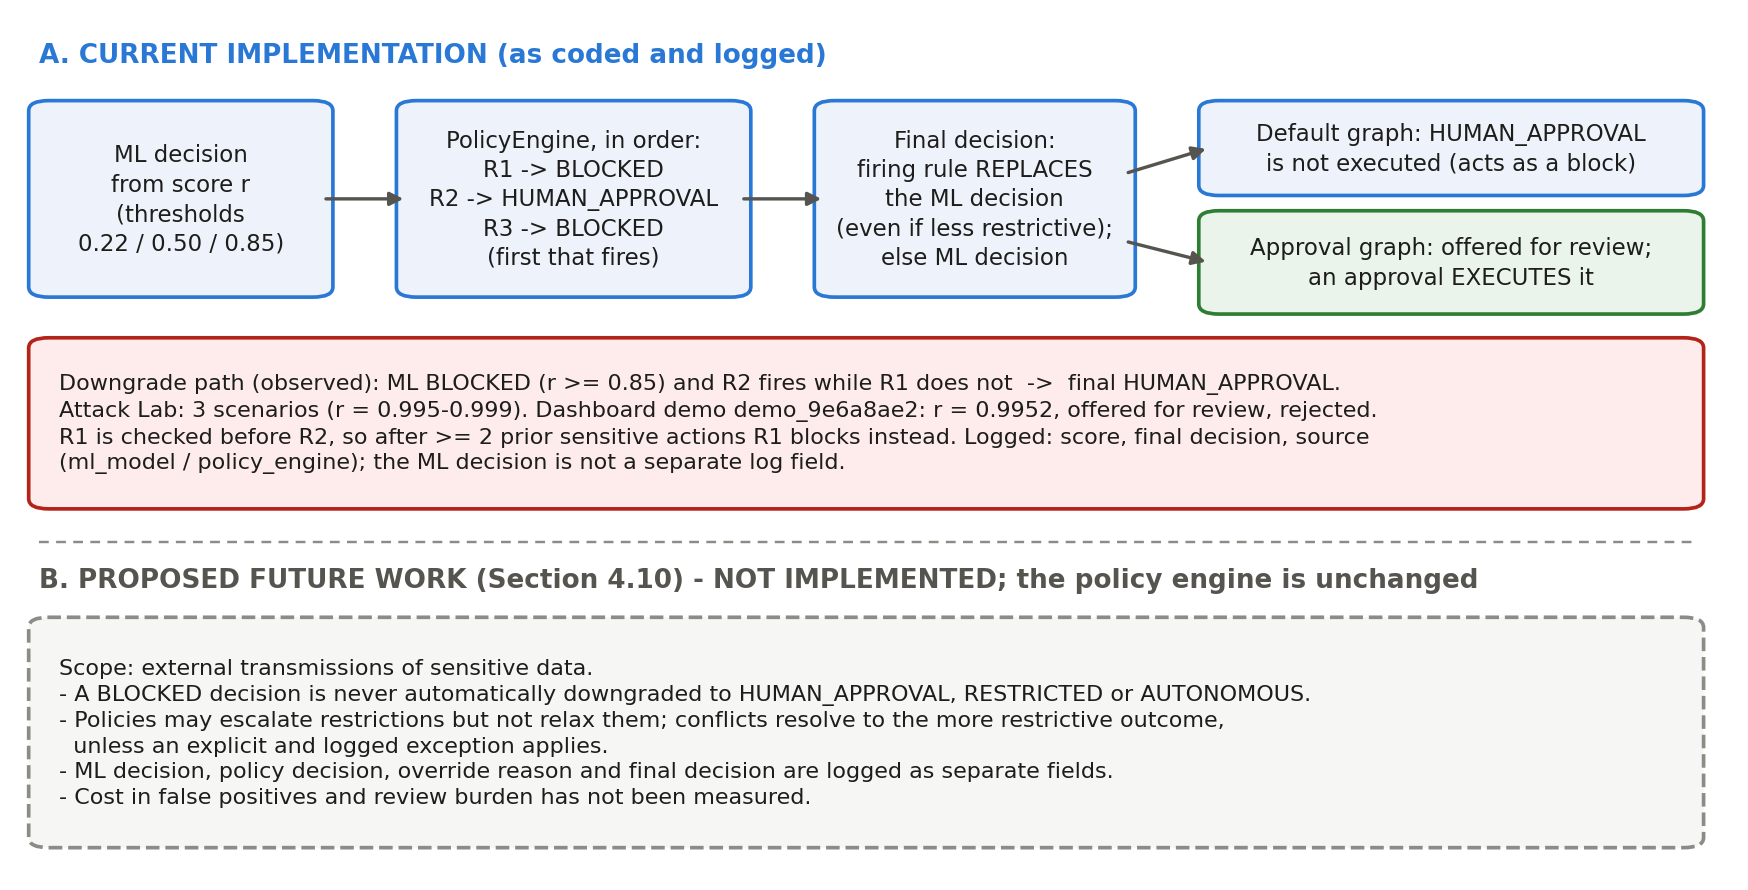
\includegraphics[width=0.85\linewidth]{figures/r04_decision_precedence.png}
\caption{(v1 Figure 2) Decision precedence. (A) Current implementation: a firing policy rule replaces the ML decision, so R2 downgrades an ML BLOCKED to HUMAN\_APPROVAL when R1 does not fire; in the approval graph that action becomes executable after approval. (B) The invariant proposed in v1, scoped to sensitive external transmissions; implemented in v2 as \code{max_severity}.}
\end{figure}

\textbf{A policy rule can downgrade a stronger ML decision.} Because a firing rule replaces the ML decision, R2 turns an ML \textbf{BLOCKED} into \textbf{HUMAN\_APPROVAL} when R1 does not fire. R1 is checked first, so after two or more prior sensitive actions, R1 blocks instead. We observed the downgrade in two places:

\begin{itemize}
\item In the Attack Lab replay, in three scenarios (\code{prompt_injection} step 5, \code{tool_poisoning} step 4, \code{data_exfiltration} step 3), with ML scores of 0.995--0.999.
\item In the persisted approval log of a dashboard demo run (\code{demo_9e6a8ae2}, scenario ``HR summary, analyst declares sensitive''). The ML score was 0.9952, above the BLOCKED threshold of 0.85. The final decision was HUMAN\_APPROVAL from \code{policy_engine}, and the action was \textbf{offered for review}. The reviewer rejected it, so nothing was sent; an approval would have executed it.
\end{itemize}

\textbf{Why it matters.} In the default graph, HUMAN\_APPROVAL is not executed, so the downgrade has no effect. In the approval graph, it turns a model block into a human decision.

For Experiment 5's two policy-escalated scenarios, the ML score was not stored. Whether they involved an ML BLOCKED therefore cannot be verified from the results (Section 9).

\textbf{Finding.} Combining a learned classifier with deterministic policy rules does not automatically produce a safer system. How the two decisions are combined is itself a security-relevant design choice, and in PrivAgent's current precedence a rule written to \emph{add} oversight (R2) can \emph{remove} a block.

\textbf{Trade-offs in choosing a precedence.} We do not claim that ``the most restrictive decision always wins'' is correct in every deployment:

\begin{itemize}
\item \textbf{False positives.} Strict precedence inherits every false positive from both components. The deployed model already raises run-level false alarms on 3.7--5.3\% of benign runs (Table 6), and a rule set adds its own.
\item \textbf{Usability and review burden.} Routing more actions to BLOCKED or HUMAN\_APPROVAL can stop legitimate work. A heavy review load also invites the approve-everything behaviour that Section 7.3 shows can be worse than no review [Parasuraman and Riley].
\item \textbf{Security-critical actions.} For irreversible actions such as an external transmission of sensitive data, letting a rule relax a high-confidence model block is hard to justify. For low-impact, reversible actions, a rule that sends a model block to review may be an acceptable usability trade-off.
\item \textbf{Privilege escalation.} Any path that relaxes a block is a target. An attacker who can shape the inputs that make a weaker rule fire first may be able to turn a block into an approvable request.
\item \textbf{Conflicting signals.} When the model and the rules disagree, the disagreement is itself informative. Discarding one decision silently hides it from reviewers and from later audit.
\end{itemize}

Whatever precedence is chosen, it should be explicit, and the ML decision, the policy decision, the override reason and the final decision should be logged as separate fields. \emph{[Editor's note (v2): v1 logged only the score, the final decision and its source; v2 logs the model decision, the fired rules and the precedence mode separately.]}

\emph{[Editor's note (v2): the invariant proposed here in v1 is implemented in v2 as \code{max_severity} precedence, and its reviewable variant is the primary configuration; ML and policy decisions are logged separately (main text Section IV-C; H1).]}

\section*{S8. Detailed comparison with Wang et al. (moved from v1 Section 2.3)}

\begin{quote}\small \emph{Editor's note (v2): this block is moved verbatim from the v1 paper and describes the \textbf{v1 system and Phase 1}. Where v2 changed the system, see TABLE II of the main text; specific rescoping notes are inline. Section, table and figure numbers inside the block refer to the v1 paper.}\end{quote}

\subsubsection*{2.3 Runtime policy enforcement for MCP-based agents (Wang et al.)}

Wang, Zhu and Li [Wang et al.] (\emph{Electronics}, 2026, published 27 June 2026) is the closest published work to PrivAgent's tool-call governance. We read the full article.

\textbf{Their system.} A single-agent \textbf{Policy Enforcement Point (PEP)}:

\begin{itemize}
\item intercepts every tool call at the tool-call boundary, after the model has chosen a tool name and arguments but before execution;
\item checks a capability token;
\item evaluates five ordered declarative rules (R01--R05; first match wins). The rules cover path scope, sensitive outbound data, high-risk tools, cross-server taint and rate caps;
\item propagates trace-level \textbf{source-integrity and data-sensitivity labels} across steps (a LabelTracker; sensitivity is ``sticky'' once detected by regex);
\item writes every decision to a \textbf{SHA-256 hash-chained audit log}.
\end{itemize}

\textbf{Their evaluation.} It uses \textbf{real LLMs}:

\begin{itemize}
\item 1,050 LLM-driven runs with deepseek-v4-pro on a 30-task controlled dataset;
\item cross-model observations on four further backends;
\item an exploratory AgentDojo pilot;
\item a scripted mode.
\end{itemize}

The full system reduced attack success from 40.0\% to 5.0\%, against 35.0\% for the strongest prompt-only baseline. Disabling cross-step labels raised call-level false negatives by 26.4 points. Tools are mostly in-process mocks, plus a preliminary validation over a real MCP stdio filesystem server. The authors frame their results as mechanism-coverage evidence on a controlled benchmark, not a deployability claim.

\textbf{Overlap with PrivAgent.} Both papers:

\begin{itemize}
\item intercept at the tool-call boundary;
\item carry information across steps to judge an outbound action;
\item use deterministic rules;
\item log every decision.
\end{itemize}

The problem spaces overlap, but the research questions differ:

\begin{itemize}
\item Wang et al. ask whether a deterministic enforcement point reduces attack success for real LLM agents.
\item PrivAgent asks how a \emph{learned} trajectory detector behaves under evaluation correction and on unseen attack patterns, and what instrumentation, rules and human review add around it.
\end{itemize}

The two evaluations therefore measure different things, and their numbers are not directly comparable.

\textbf{Differences:}

{\footnotesize
\setlength{\tabcolsep}{3pt}
\begin{longtable}{>{\raggedright\arraybackslash}p{0.130\dimexpr\linewidth-6\tabcolsep\relax}>{\raggedright\arraybackslash}p{0.435\dimexpr\linewidth-6\tabcolsep\relax}>{\raggedright\arraybackslash}p{0.435\dimexpr\linewidth-6\tabcolsep\relax}}
\hline
\textbf{Aspect} & \textbf{Wang et al. [Wang et al.]} & \textbf{PrivAgent} \\
\hline
\endhead
Architecture & single agent loop with one enforcement point & LangGraph multi-agent orchestration (four roles), with agent-to-agent handoffs instrumented separately \\
Cross-step signal & propagated SI/DS labels, \textbf{enforced} & a learned trajectory score over count/maximum features, \textbf{enforced}; per-item provenance labels, \textbf{shadow only} (v1); enforced in v2 \\
Rules & five rules, first match & three rules; v1: a firing rule replaces the ML decision; v2: rules only escalate \\
Audit & hash-chained, tamper-evident & v1: append-only by convention; v2: hash-chained \\
Human confirmation & REQUIRE\_CONFIRM is treated as a block (no confirmation channel) & an opt-in pause-and-review workflow with an execution ledger \\
LLMs & real LLMs (deepseek-v4-pro, four more backends) & v1: scripted LLM only; v2: one local 3B model (pilot) \\
MCP & mock tools plus a preliminary real stdio filesystem server & four locally run FastMCP stdio server processes, synthetic data, scripted workloads \\
Evaluation & attack success, task success and false-positive/false-negative rates over LLM-driven runs & v1: step-level detection metrics on synthetic trajectories; scripted demonstrations; v2 adds canary-based attack success on scripted graph scenarios and a 3B-model pilot \\
\hline
\end{longtable}}

PrivAgent's v1 evaluation was weaker in realism: no real LLM, synthetic trajectories, and a scripted workload, and v1 lacked a tamper-evident audit log. \emph{[Editor's note (v2): v2 adds a hash-chained log and a small real-LLM pilot; the realism gap to Wang et al. remains (one 3B model, scripted family B writer).]} Its narrower contribution is a more detailed account of how a learned trajectory detector can be inflated by leakage and shortcuts. We make no claim that PrivAgent outperforms Wang et al. on any measure.

\section*{S9. Development results (not confirmatory)}

Development data only (WP1--WP6, before the freeze). Each row is quoted from the claim--evidence ledger (\code{research_paper/v2/CLAIM_EVIDENCE_LEDGER_v2.md}), with its artifact, commit and status.

{\footnotesize
\setlength{\tabcolsep}{3pt}
\begin{longtable}{>{\raggedright\arraybackslash}p{0.060\dimexpr\linewidth-12\tabcolsep\relax}>{\raggedright\arraybackslash}p{0.284\dimexpr\linewidth-12\tabcolsep\relax}>{\raggedright\arraybackslash}p{0.076\dimexpr\linewidth-12\tabcolsep\relax}>{\raggedright\arraybackslash}p{0.284\dimexpr\linewidth-12\tabcolsep\relax}>{\raggedright\arraybackslash}p{0.060\dimexpr\linewidth-12\tabcolsep\relax}>{\raggedright\arraybackslash}p{0.284\dimexpr\linewidth-12\tabcolsep\relax}}
\hline
\textbf{\#} & \textbf{Claim} & \textbf{Planned location} & \textbf{Supporting artifact} & \textbf{Commit} & \textbf{Status} \\
\hline
\endhead
D1 & WP1 (dev: train, val, variant C; seeds 42, 7, 1234): \code{max_severity} 0 downgrades in every set; \code{first_fire_v1} 206 / 53 / 80; \code{max_severity_reviewable} 168 / 43 / 66, none to allowed & \S{}4.13 & \code{experiments/v2/results/precedence_ablation_dev.md} & \code{bb9d53a} & VERIFIED-FILE \\
D2 & WP1 (dev): benign cost differences \code{max_severity} $-$ \code{first_fire_v1} and \code{max_severity_reviewable} $-$ \code{first_fire_v1} are +0.0000 [+0.0000, +0.0000] in every set (approval volume, ext. send hard-blocked, block rate, any stop) & \S{}4.13 & same & \code{bb9d53a} & VERIFIED-FILE \\
D3 & WP2 (dev, live replay scenarios): scoring handoffs turns \code{hr_exfil_misreported} and \code{finance_exfil_misreported} from AUTONOMOUS/transmitted to BLOCKED/not transmitted; Attack Lab outcomes identical across v2 modes; \code{path_cross_agent_leak} missed in every mode & \S{}4.14 & \code{experiments/v2/results/handoff_scoring_dev.md} & \code{a6f7fcc} & VERIFIED-FILE \\
D4 & WP2 (dev): every live handoff pseudo-action tuple appears in the seed-42 training data (25,841 rows) & \S{}4.14 & same, coverage table & \code{a6f7fcc} & VERIFIED-FILE \\
D5 & WP3 (dev): the RESTRICTED semantics escalate 0 of 1,059 benign validation runs (3 seeds) & \S{}4.15 & \code{experiments/v2/results/restricted_semantics_dev.md} & \code{468aec4} & VERIFIED-FILE \\
D6 & WP3: hash-chained logs, HKDF key separation, send binding implemented and tested & \S{}4.15 & WP3 code and tests (\code{experiments/v2/WP3_DIFF.patch}) & \code{468aec4} & TEST-15NOV (code not re-read for this ledger) \\
D7 & WP4 (dev half, 24 scenarios $\times$ 5 declarations): H3 shadow 15/40 attack sends vs enforce (primary v2) 0/40; benign completed 30/65 vs 10/65; accurate declaration identical (3 completed / 8 review / 2 hard-blocked of 13) & \S{}4.16 & \code{experiments/v2/results/wp4_dev.md}; \code{experiments/v2/MORNING_REPORT.md} \S{}3 & \code{c453674} & VERIFIED-FILE \\
D8 & WP4 (dev): score with R1 on stops 40/40 attacks but completes 10/65 benign sends (50 hard-blocked) & \S{}4.16 & \code{wp4_dev.md} per-condition table & \code{c453674} & VERIFIED-FILE \\
D9 & WP5 (dev, validation split, 10 seeds): AUPRC 0.968 [0.965, 0.971], step recall 0.957; seed-42 thresholds reproduce \code{models/thresholds.json} & \S{}7.7 & \code{experiments/v2/results/multiseed_dev.md} & \code{89bbe1b} & VERIFIED-FILE \\
D10 & WP6 (dev smoke, qwen2.5:3b, 6 tasks, family A): 0 of 18 attack runs attempted a send & \S{}7.7; \S{}9.x & \code{experiments/v2/results/real_llm/smoke_ollama_qwen2.5-3b_20261115T035239.md} & \code{c453674} & VERIFIED-FILE \\
D11 & WP6 (dev, family B smoke, 36 runs): 2 runs failed before the writer from an empty \code{search_queries} list (\code{IndexError}), originally recorded as exclusions; reclassified as model failures (\code{adc18b0}) & \S{}7.7 & \code{experiments/v2/results/real_llm/smoke_ollama_qwen2.5-3b_ts2-B_20261115T132601.md}; pre-registration third revision & \code{adc18b0} & VERIFIED-FILE \\
D12 & WP4 (dev): governance makes identical decisions for legitimate sensitive sends and for attacks carrying the same data, so a reviewer gets no signal from the system to tell them apart & \S{}VII & \code{experiments/v2/MORNING_REPORT.md} \S{}6; \code{experiments/v2/results/wp4_dev.md} & \code{c453674} & VERIFIED-FILE (stated in the development report; not separately recomputed) \\
\hline
\end{longtable}}

\section*{S10. Exploratory analyses: per-task table}

The per-task outcome table for the \code{v2} family B runs (EXPLORATORY, not pre-registered) is in \code{experiments/v2/exploratory/EXPLORATORY_v2_familyB_and_H4b.md}, Section 1.

\section*{S11. Claim--evidence mapping of the main text}

Every number in the main text cites a ledger row in an HTML comment. This table lists, per section, the rows cited (generated from the manuscript). The full ledger, with artifacts, commits and statuses, is \code{research_paper/v2/CLAIM_EVIDENCE_LEDGER_v2.md}; \texttt{v1:\#N} is row N of \code{research_paper/final/CLAIM_EVIDENCE_LEDGER.md}.

{\footnotesize
\setlength{\tabcolsep}{3pt}
\begin{longtable}{>{\raggedright\arraybackslash}p{0.406\dimexpr\linewidth-4\tabcolsep\relax}>{\raggedright\arraybackslash}p{0.594\dimexpr\linewidth-4\tabcolsep\relax}}
\hline
\textbf{Manuscript section} & \textbf{Ledger rows cited} \\
\hline
\endhead
Title and Abstract & v1:\#1, P1, S2, V1, C3, C4, C7, C8, C10, C11, C15, C24, S8, C12, C13 \\
I. INTRODUCTION & S1, P1, S2, V1, v1:\#12, C20, C12, v1:\#22, v1:\#23, C3, C4, C2, C5, S4, C7, C8, S13, C10, C11, C24, X2, C13b \\
II. RELATED WORK & v1:\#40, S8, L1, S4, S5, S6, S7 \\
III. THREAT MODEL & S2, S8, C22 \\
IV. PRIVAGENT DESIGN & S1, S4, S5, S6, S7, S14, v1:\#20, v1:\#9, v1:\#19, S13, S8, v1:\#37, v1:\#21, v1:\#26, v1:\#29, v1:\#30, v1:\#31 \\
V. STUDY DESIGN & S7, S8, S10, C21, S2, P1, V1, v1:\#18, v1:\#19, S4, S5, S9, S11, S3, S12, P4, P3, P2, P5 \\
VI. RESULTS & v1:\#1, v1:\#2, v1:\#9, v1:\#11, v1:\#3, v1:\#4, v1:\#5, v1:\#6, v1:\#12, v1:\#17, v1:\#22, v1:\#23, v1:\#27, v1:\#34, C3, C1, C2, C5, C4, C4b, C7, C8, S7, C9, C10, C11, C14, C12, C13, C13b, C16, C17, C15, C24, S8, C18, C18b, C18c, C19, S10, C20, V1, X1, X2, X4, X3 \\
VII. DISCUSSION & C15, C24, C12, C20, C10, C7, C8, S13, C2, C3, C4, C5, S4, X2, v1:\#34, D12, C11, C13, C13b, X3 \\
VIII. LIMITATIONS AND THREATS TO VALIDITY & S10, S8, C21, C22, S7, X2, S3, C14, S2, C13b, v1:\#16, V1, v1:\#37, v1:\#42 \\
IX. CONCLUSION & C24, C12, C10, C11, C7, C8, C4, C5, C15, S8, C13 \\
\hline
\end{longtable}}

\section*{S12. Reference verification}

{\footnotesize
\setlength{\tabcolsep}{3pt}
\begin{longtable}{>{\raggedright\arraybackslash}p{0.281\dimexpr\linewidth-6\tabcolsep\relax}>{\raggedright\arraybackslash}p{0.359\dimexpr\linewidth-6\tabcolsep\relax}>{\raggedright\arraybackslash}p{0.359\dimexpr\linewidth-6\tabcolsep\relax}}
\hline
\textbf{Reference} & \textbf{Checked against (17 Nov 2026 unless stated)} & \textbf{Status} \\
\hline
\endhead
CaMeL & \url{https://arxiv.org/abs/2503.18813}; \url{https://www.computer.org/csdl/proceedings-article/satml/2026/785900a587/2jZks3ksGT6} & arXiv record verified. Venue: Proc. IEEE SaTML 2026, verified by the author in a browser on 17 Nov 2026 (the CSDL page does not render for automated fetching). Pages \textbf{[VERIFY]} \\
FIDES & \url{https://neurips.cc/virtual/2026/poster/152696}; \url{https://arxiv.org/abs/2505.23643} & NeurIPS 2026 (title and authors as on the conference page); page numbers not available \\
Permissive IFC & \url{https://arxiv.org/abs/2410.03055}; \url{https://www.microsoft.com/en-us/research/publication/permissive-information-flow-analysis-for-large-language-models/} & TMLR, Oct. 2025, as listed by Microsoft Research (per the authors' instruction); the OpenReview page (id ufYRO8y3mr) could not be read \\
CapAgent & \url{https://api.crossref.org/works/10.3390/bdcc10090293} & verified (Crossref); publisher page returned HTTP 403 \\
Arp et al. & \url{https://www.usenix.org/conference/usenixsecurity22/presentation/arp} & verified \\
TESSERACT & \url{https://www.usenix.org/conference/usenixsecurity19/presentation/pendlebury} & verified \\
AgentLeak & \url{https://api.crossref.org/works/10.1109/ACCESS.2026.3704541}; \url{https://arxiv.org/abs/2602.11510} & verified \\
GuardAgent & \url{https://proceedings.mlr.press/v267/xiang25a.html} & verified \\
ShieldAgent & \url{https://proceedings.mlr.press/v267/chen25ae.html} & verified \\
Kairos & \url{https://arxiv.org/abs/2610.18457} & verified; identity confirmed by the authors \\
Noumi et al. (Inspectra) & \url{https://arxiv.org/abs/2608.21423} & verified (title, authors, submission date; the abstract names Inspectra as the authors' platform) \\
McNemar & \url{https://api.crossref.org/works?query.bibliographic=McNemar}... (DOI 10.1007/BF02295996) & verified (Crossref) \\
Claude Code (AI system, cited in Sections I--IX) & \url{https://code.claude.com/docs/en/overview} & page title and product name verified \\
DeLong et al. & Crossref (DOI 10.2307/2531595) & verified except the end page (Crossref gives the first page only) \textbf{[VERIFY]} \\
All other references & carried from the v1 paper, whose ledger records them as LIT (v1 ledger rows 40, 41) & not re-checked in this pass \\
\hline
\end{longtable}}

\end{document}
